Nick Vosseteig

2014-10-03

Set up, helping other teams, and finding materials.

\begin{tabular}{|p{5cm}|p{5cm}|}
 \hline
 Set up&
One thing we did this week was set up Miktex and GitHub, and moved over the other engineering notebooks that we had written beforehand into the new system. We now have everything set up and engineering notebooks in the future will be easier to format/create.
 \\
 \hline
Helping other teams&
Since there are two other less experienced teams at our school, this week I also helped them set up the programs that they needed to test out some of the things they had built for their robot. Most were unfamiliar with RobotC, so I helped them to write basic programs.
 \\
 \hline
 Finding materials&
We decided to buy some surgical tubing this week so that we can start building a prototype of the launcher next week.
 \\
 \hline
\end{tabular}

\section*{Miktex and Github}
This week the main thing we worked on was setting up Miktex and Github so that we can format our engineering notebooks in a more consistent and better format.

\section*{Helping other teams}
The other thing I did this week was help the other teams program their prototypes for certain parts. This was hard because none of them had any experience with programming previously. I managed to help them write some code that allows them to control the motors on their robot with the Logitech controllers.

The last thing we did was come up with a basic design for the launcher and tube mechanism that we plan to build with the surgical tubing we are going to buy.

\begin{center}
 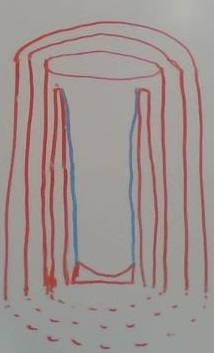
\includegraphics[width=10cm]{./Entries/Images/launcher.png}
 %launcher.png: 740x709 pixel, 90dpi, 20.89x20.01 cm, bb=0 0 592 567
\end{center}
